\section{Controller}
Our first idea for implementing the controller was to detect the position of the shape relative to the position of the camera and so move the camera in the good position. However, this model had some default which could have take time to correct. Indeed, it's  difficult to get the 3D position of something in a 2D picture. The depth of the picture can give differents position even if we need to do the same move in order to center it.

\begin{figure}[!ht]
 \begin{minipage}{0.49\textwidth} % il faut un plus petit que la page elle même pour eviter l'overbox
\begin{center}
 
\includegraphics[width=\textwidth]{depth1.png}
    \label{titiecrase}
\end{center}
 \end{minipage}
 \begin{minipage}{0.49\textwidth}
 \begin{center}
    
\includegraphics[width=\textwidth]{depth2.png}
    \label{bochateau}
 \end{center}
 \end{minipage}
\caption{2 pictures with same angle movement needed}
\end{figure}

One other problem was the accuracy of the encoder. In fact, the encoder are physically not well attach to the camera and so we can easily get errors on our final position. Because of this problems, we need a strong controller even if the system to control is simple.

\subsection{Our solution}
In order to a avoid such kind of problems, we decided to use a different model of controller. We don't use the encoder as feedback but only the camera. We have so a simple controller that take the position from the camera and move in the right direction with a speed depending of how far is the shape from the center. Furthermore, our hand movement for moving the shape is smooth and can be easilly controlled by a simple proportionnal controller.

\begin{figure}[!ht]
\centering
 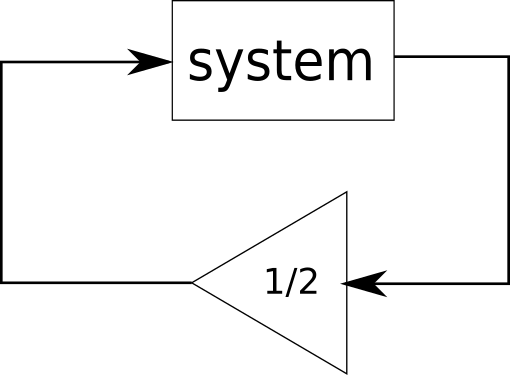
\includegraphics[width=0.7\textwidth]{controller.png}
 \caption{Controller schematic}
 \label{contr_sche}
\end{figure}

\subsection{Implementation Nios vs Overo}

As see before, our controller is very simple. We get an int value from the camera coressponding to the pixel center and we only divide it by a factor of 2 in order to eliminate echo and we convert it into a value between 0 and 100 which correspond to the duty cycle. Because of we are using a gain of 1/2, speed is not the most important part and we convert final value to an integer so that accuracy is not so important. In our case, the most important criterion was time implmeentation because the deadline was coming soon. We so decided to implement it in the overo fire because we were sure to be able to implement and fix it quickly contrary to use the nios core. Indeed, we experimented this semester that a new hardware always took more time than expected because of various problems like communication, or wrong documentation.

\begin{figure}[!ht]
\hspace{-1cm}
\begin{tabular}{|c|c|c|c|c|c|c|}\hline
                         & Accuracy  & Implementation & Flexibility & Real-time & Ressources & result \\\hline
coefficient   &         1          &           3                      &         2           &           1         &           1            &              \\\hline
Overo            &      ++          &            ++                    &        ++           &        -         &           +           &    12        \\\hline
Nios               &      ++         &              -                &         -       &         +          &           +        &   -1 \\\hline
\end{tabular}
\caption{trade-off table of controller unit between Nios and Overo}
\end{figure}
